\chapter{FG Nup aggregation under crowded conditions}\label{ch05}

While our bound-state diffusion model of selectivity is general enough to apply to many biofilters, we have been using the nuclear pore in particular as inspiration.  We predict that its selective properties arise from the continued mobility of transport factors while bound to FG Nups.  One mechanism of bound-state diffusion arises from the flexible, tether-like nature of the disordered Nups.  Such a mechanism is possible whether the Nups form a polymer brush or a transient hydrogel, so long as they remain sufficiently dynamic.

The exact conformation of Nups within the nuclear pore is unknown, due to the difficulty in imaging such a disordered system.  Some Nups, such as Nsp1, aggregate in buffer to form hydrogel structures \cite{frey06, frey07, ader10}, although evidence suggests it does not aggregate in the cellular environment \cite{hough15}.  Other Nups can form phase-separated liquid droplets \cite{schmidt15}.  Nup153 forms amyloid fibrils \textit{in vitro} (Fig.~\ref{fig:amyloid}B) at a rate which is increased by the addition of inert crowders \cite{milles13}.  Amyloid structures, as shown in in Fig.~\ref{fig:amyloid}A, are long chains of stacked $\beta$ sheets which are much less flexible and dynamic than individual disordered proteins, potentially limiting the effectiveness of the tethered bound diffusion of transport factors.  Amyloid fibrils are commonly formed by disordered proteins upon aggregation and are often implicated in disease \cite{jahn08}.    On the other hand, atomic force microscopy (AFM) data and simulations suggest that Nups in the nuclear pore remain highly dynamic \cite{sakiyama16,moussavi-baygi16}.

We decided to test the aggregation behavior of a fragment of the essential FG Nup Nsp1 known as FG124, described in Sec.~\ref{sec:Nups} and Appendix~\ref{appx:sequences}.  This 124-amino-acid peptide contains eight FG motifs and is known to aggregate in buffer over the course of several hours.  However, in-cell NMR shows it to remain disordered inside bacterial cells \cite{hough15}.  Given the disparity in aggregation behavior under these different conditions, we wanted to determine whether we could encourage or suppress aggregation and amyloid formation with our choice of crowding agents.

\begin{figure}
\caption[Aggregation of FG Nups into amyloid fibrils.]{Aggregation of FG Nups into amyloid fibrils. (A) Schematic of possible aggregation states of a disordered protein, including disordered aggregates, intermediate amyloid-like states, and fibrils composed of stacked beta-sheets. Rectangles denote secondary structure.  Figure adapted from \cite{jahn08}. (B) Negative-staining electron micrograph of amyloid fibrils consisting of the human Nup153 FG domain.  Arrows indicate characteristic twists of the fibrils.  Figure adapted from \cite{milles13}.}
\centering
\includegraphics[width=\textwidth]{figs/ch05/amyloid-intro}
\label{fig:amyloid}
\end{figure}

While the simplicity of studying aggregation of FG124 in buffer alone is appealing, the nuclear pore is a very different environment.  Cells are extremely crowded with proteins, nucleic acids, and other macromolecules.  Some estimate that macromolecules fill 30\% of a cell's volume \cite{breydo14}.  Crowding can have strong effects on a protein's behavior, sometimes in surprising ways.  Furthermore, crowding effects can differ depending on whether the crowders are inert, interacting, compact, extended, and so on.  Generally speaking, crowding seems to increase the rate of aggregation of disordered proteins, but this is by no means universal \cite{breydo15, breydo14,lee12,magno10,milles13}.  The presence of small crowders tends to encourage proteins to take on compact conformations due to the excluded volume effect, which in the case of IDPs often leads to aggregation.  However, the viscosity changes due to crowding may inhibit the formation of aggregates \cite{sleutel12,saha16}.  Crowding with proteins capable of nonspecific interactions has been shown to inhibit the partitioning of IDPs into phase-separated liquid droplets \cite{protter18}.  Other important but not well-understood factors include crowder structure and interactions, agitation or its absence, and the presence of an air-water interface \cite{lee12, breydo14}.

We studied FG124 aggregation in the presence of various crowding agents, both inert and nonspecifically interacting, using a number of techniques.  The kinetics were probed with a fluorescence aggregation assay, which showed significant differences between crowders.  Two inert crowders, poly(ethylene glycol) and polyvinylpyrrolidone, were chosen for further NMR and fluorescence spectroscopy.  The results do not have a clear interpretation but suggest that the presence and type of crowding agent is indeed affecting the local chemical environment of the peptide's residues, including its phenylalanines.  Given the importance of the FG repeats to Nup cohesiveness and transport factor binding, this could have implications for the optimal conditions under which to study Nup behavior in vitro.

\section{Fluorescence time courses}

In order to probe the aggregation kinetics of FG124, we incubated samples in the presence of crowders and thioflavin T (ThT), a dye which is sensitive to the presence of amyloids.  Over the course of several hours, FG124 aggregated and the fluorescence intensity from ThT increased.  By recording the intensity at 10-minute intervals, we were able to plot sigmoidal aggregation curves for the samples, as shown in Fig.~\ref{fig:sigmoid-fit}.  These curves show a lag phase while the aggregates are nucleating, followed by a growth phase of rapid aggregation, ending in a plateau phase.  We recorded timecourses for multiple crowders, including inert crowders as well as nonspecifically binding ones, and analyzed the resulting aggregation parameters.  Poly(ethylene glycol) (PEG) and polyvinylpyrrolidone (PVP) were chosen as representative inert crowders.  Cell lysate was used to imitate the cellular environment and test the effect of nonspecific interactions on FG124 aggregation.  Finally, serine was used as a crowder as previous work demonstrated that it caused Nup153 to aggregate more quickly \cite{milles13}.  Many of the timecourse experiments were performed by Sophie Reskin and Paul Marchando, and Sophie also took part in the analysis.

Thioflavin T is a dye that grows much brighter when bound to amyloids.  Upon binding, its absorption maximum shifts from from 385 nm to 450 nm and its emission maximum from 445 nm to 482 nm \cite{picken12}.  Although ThT is a more reliable indicator of amyloids than other fluorescence methods, notably Congo red stain, it suffers from reproducibility problems.  There is no consensus on the mechanism of ThT binding to amyloids.  Some proposed mechanisms rely on the presence of ThT micelles, which form above a critical concentration of about 4 um, while others advocate for avoiding micelles \cite{khurana05, groenning09}.  There is some evidence that amyloid fibrils can adsorb to the plastic surface of a multiwell plate, decreasing ThT fluorescence intensity as the fibrils mature \cite{murray13}.  Often in our timecourse experiments, the ThT fluorescence did reach a maximum and then decrease.  The fluorescence intensity also depends on the sample viscosity, an effect which we noticed in our timecourses \cite{sulatskaya10}.  Despite these challenges, thioflavin T is the most reliable dye for detecting the process of amyloid formation.

%basename = '/Users/lauramaguire/Google Drive/Hough Lab/Nuclear Pore Team/Data/FG124 aggregation timecourses/';
% Date in 'yymmdd' format
%date = '170126';
%13% PEG rep 3
\begin{SCfigure}
\caption[Sample sigmoid fit to FG124 aggregation timecourse.]{Sample sigmoid fit to FG124 aggregation timecourse with 13\% w/v PEG.  Burst phase and stationary phase are shown; lag phase took place before data collection began.  Fit is to Eqn.~\ref{eq:sig-fit}.\\}
\centering
\includegraphics[width=0.5\textwidth]{figs/ch05/sample-sigmoid}
\label{fig:sigmoid-fit}
\end{SCfigure}

\subsection{Methods}

\subsubsection{Buffers} Potassium transport buffer (PTB) (150 mM KCl, 20 mM HEPES, 2 mM $\tx{MgCl}_2$) was used for all timecourse and NMR samples.

\subsubsection{FG124 preparation} His-tagged FG124 was expressed in \textit{E. coli} in the plasmid pRSF.  Cultures were grown in LB and  induced at 37$^\circ$C for 2-4 hr with 1 mM IPTG at OD 0.6-0.8.  Periplasmic matrix was removed prior to lysis.  Cells were then lysed via sonication and FG124 purified using TALON cobalt resin (Appendix~\ref{appx:protein-purification}).  All purification buffers were PTB with 7M guanidine hydrochloride (GuHCl) and 1:1000 protease inhibitor cocktail (PIC).  The elution buffer also contained 250 mM imidazole.

\subsubsection{Timecourse preparation} Stocks of PEG (avg. MW 20 kDa, Sigma, Bio-Ultra) and PVP (avg. MW 40 kDa, Sigma) in PTB were prepared at 20 or 40\% w/v; L-serine (EMD Millipore Calbiochem) stocks were prepared at 30\% w/v.  PEG and serine were at pH 7; PVP was pH 7 or pH 5.  Lyophilized lysate was prepared by homogenizing BL21 DE3 Gold cells and centrifuging them.  The supernatant was lyophilized in a decomposing 25 mM ammonium bicarbonate buffer and resuspended in PTB to the desired concentration when needed.  A 10 mM stock solution of ThT in PTB was prepared and filtered no more than a week before the timecourse, stored at room temperature and protected from light.  Immediately prior to starting the timecourse, FG124 was desalted into PTB to remove the imidazole and GuHCl.  Samples were promptly prepared containing the appropriate percentage of crowder, a final concentration of 0.3-2.5 mg/mL FG124, and 200 $\mu$M ThT.  All samples in the same timecourse had the same concentration of FG124, including the buffer sample, which contained no crowding agent.  Blanks were prepared with crowding agent and ThT, but no FG124.  Samples were pipetted into black, flat-bottomed, clear-bottomed 96-well plates with 150 $\mu$L per replicate.  Each sample yielded four to six replicates.  Only one blank replicate was used per condition.  One negative control and corresponding blank were prepared per timecourse containing 7M GuHCl and no crowding agent but using the same protein sample as all other conditions.  Each well contained a 3mm-diameter glass or Teflon bead.  The plate was sealed with a PCR seal and taken to a Safire II plate reader.  The fluorescence was measured from the bottom at 10-minute intervals with an excitation wavelength of 450 nm, emission wavelength of 482 nm, and 5 nm bandwidths.  The plate shook orbitally at high speed between measurements and was held at a temperature of 30$^\circ$C.  The time between desalting and beginning the plate reader measurements was typically about an hour; the time of desalting was taken as $t=0$ for the purposes of calculating lag time. In parallel with the sample preparation, the concentration of the desalted FG124 was measured with a BCA assay.  Sophie Reskin helped to optimize this assay, making extensive use of \cite{giehm10}.

\subsubsection{Timecourse analysis}

After carrying out the aggregation timecourse, the data were normalized and fit to a sigmoid function in order to extract aggregation lifetimes and lag times.

The data were first normalized to the blanks, which contained crowding agents but no protein.  In nearly all cases, the blank intensity remained steady over time, as expected.  In those cases, the mean blank intensity was subtracted from the corresponding data.  In cases where the blank intensity changed over time, it was subtracted pointwise from the data.

Then the normalized curves were fit to a sigmoid given by
\begin{equation}
I(t) = C + \frac{A}{1+\exp \left(-k(t-T_{1/2})\right)}
\label{eq:sig-fit}
\end{equation}
where $I(t)$ is the normalized fluorescence intensity as a function of time (Fig.~\ref{fig:sigmoid-fit}).  The aggregation dynamics are described by the rate $k$ and the half-time $T_{1/2}$, which reflects the time needed for the intensity to reach half of its asymptotic value.  More descriptive than the half-time is the lag time $T_\ell$, calculated as
\begin{equation}
T_l = T_{1/2} - \frac{2}{k}
\end{equation}
and representing the duration of the lag phase \cite{arosio15}.  The lag time here is defined as the intersection of the tangent line of maximum slope of the growth phase with the flat background signal of the lag phase.  

The offset $C$ and final amplitude $A$ are less meaningful in this context, and less reliable.  The offset should in principle be $C=1$, as the fluorescence of the sample and its blank should be equal before aggregation has begun.   Experimentally, $C \sim$ 1-2, reaching a maximum near $C= 10$ for a few sample conditions.  While this may have been because sample aggregation had already begun, the long lag times of those conditions do not support that interpretation.  It is possible that the presence of the unaggregated protein caused a change in baseline fluorescent through an unknown mechanism.

The plateau phase asymptotes to an intensity given by $I_\infty=C+A$.  We found significant variation in $I_\infty$ for the same condition between timecourses, and the relative magnitudes of different conditions also varied between timecourses.  As seen in previous ThT studies, higher viscosity tended to result in higher values of $I_\infty$. Therefore, we do not consider $I_\infty$ in our analysis, leaving the aggregation rate $k$ and lag time $T_\ell$ as parameters of interest.

Next we normalized once again to account for differences between timecourses.  It was impossible to hold the FG124 concentration exactly fixed between timecourses.  Final protein concentration varied between 0.3 and 2.5 mg/mL. Within each timecourse, we averaged the fit parameters for all replicates of FG124 in buffer only and subtracted that average from each replicate of each crowding condition.

%The final concentration of crowding agent was 19\% serine w/v, 13\% PEG, and 13\% PVP. 
% Lysate concentration varied between time courses and was in the 1-10 mg/mL range.  

\begin{figure}
\caption[Aggregation rates and lag times for all crowding agents.]{(A) Aggregation rates and (B) lag times for all crowding agents, normalized to the no-crowding condition.  Crowder concentrations were 19\% w/v serine, 13\% PEG, 13\% PVP, and approximately 10 mg/mL lysate.  Lysate concentration varied somewhat between experiments. Error bars are standard error of the mean.}
\centering
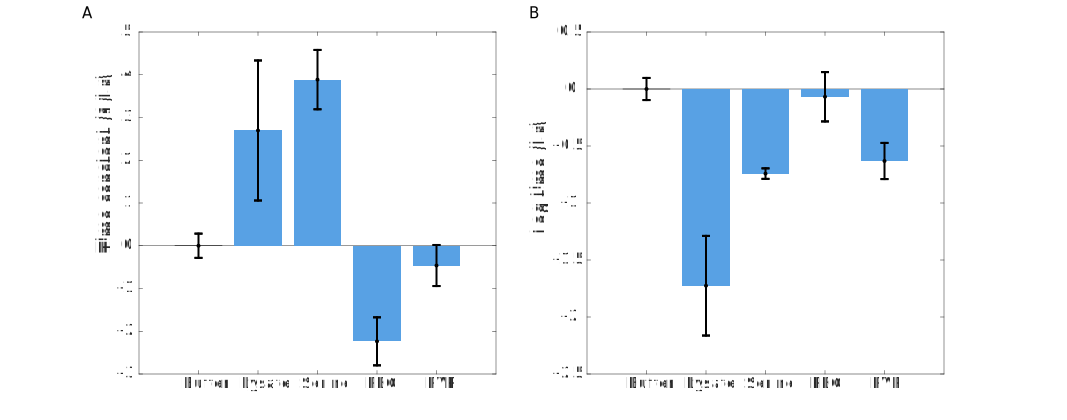
\includegraphics[width=0.8\textwidth]{figs/ch05/barCharts.pdf}
\label{fig:tht-all-conditions}
\end{figure}

% Recreating what I did to make these plots.  From Matlab script, loaded 
%j27 = load('C:\Users\bit\Desktop\sophie\time course fits\170127\170127_workspacefinal.mat');
%f19 = load('C:\Users\bit\Desktop\sophie\time course fits\170219\170219_workspace_final.mat');
%f21 = load('C:\Users\bit\Desktop\sophie\time course fits\170221\170221_workspace_final.mat');
%f28 = load('C:\Users\bit\Desktop\sophie\time course fits\170228\170228_workspace_final.mat');
%m07 = load('C:\Users\bit\Desktop\sophie\time course fits\170307\170307_workspace_final.mat');
%which desktop was this?  Probably old lab desktop

%use `dataforpaper.mat' in ch05 folder

\subsection{Results}

The mean fit parameters and number of replicates for each crowder condition are shown in Table~\ref{table:crowder-params} and Fig.~\ref{fig:tht-all-conditions}.  For both the aggregation rate $k$ and lag time $T_\ell$, a one-factor ANOVA rejected at the $p=0.05$ level the null hypothesis that there was no difference between the means.  Two-tailed t-tests were then run comparing all conditions shown in Fig.~\ref{fig:tht-all-conditions}.  The resulting $p$-values were below 0.05 except for those comparing no crowder to PVP (rate), no crowder to PEG (lag time), and serine to PVP (lag time).  All $p$-values are reported in Appendix~\ref{appx:p-values}.



\begin{table}[b!]
\centering
  \caption[Aggregation rates and lag times for all crowding agents.]{Mean aggregation rate and lag time for all crowding agents, normalized to no-crowder condition. Number of replicates is $N$. Errors are standard errors of the mean.}
    \label{table:crowder-params}
    \begin{tabular}{r |r |r| r}%{p{3cm}|p{3cm}p{3cm}p{2cm} }%p{2cm}p{2cm}}
       Condition & Rate $k$ (1/hr) & Lag time $T_\ell$ (hr)  & $N$ \\
      \hline
	No crowder & $0\pm0.3$ & $0\pm0.1$& 32\\
	Lysate & $2.7\pm1.6$  & $-1.7\pm0.4 $ & 16 \\
     	Serine (19\%)& $3.7\pm0.7$  & $-0.7\pm0.05  $& 28 \\
      	PEG (25\%) & $-1.9\pm0.4$  & $1.7\pm1.3  $ & 7 \\
     	PEG (20\%) & $-0.3\pm0.3$   & $0.8\pm0.7$  & 7 \\
	PEG (13\%) & $-2.2\pm 0.6$ & $-0.07\pm 0.2 $ & 31 \\
	PEG (5\%) & $0.2\pm1.0$  & $-0.6\pm0.3 $ & 7 \\
      	PVP (25\%) & $0.2\pm2.6$  & $2.7\pm1.2 $  & 7 \\
     	PVP (20\%) & $-1.1\pm0.5$  & $0.9\pm0.7$   & 6\\
	PVP (13\%) & $-0.5\pm0.5$  & $-0.6\pm0.2 $ & 32\\
	PVP (5\%) & $-0.9\pm0.6$  & $-0.5\pm0.3$   & 7 \\
    \end{tabular}
\end{table}

Several timecourses were run without crowders at varying pH.  Table~\ref{table:FG124-pH} shows the resulting fit parameters, given as lifetime $\tau = 1/k$ and lag time $T_\ell$.  Six replicates were run of each pH condition.  One-way ANOVAs fail to reject the null hypothesis at the $p=0.05$ level, suggesting that FG124 aggregation is not affected by pH in the range 5-8.

Two crowders, PEG and PVP, warranted special attention.  These inert crowders are commonly used interchangeably, but the results of timecourses containing 13\% PEG or PVP suggest that they may in fact affect FG124 differently (Fig.~\ref{fig:tht-all-conditions}).  In order to investigate any differences between PEG and PVP, timecourses were run with varying crowder concentrations and analyzed as before.  Mean parameter values are shown in Fig.~\ref{fig:peg-pvp}.  Statistics are given in Appendix~\ref{appx:p-values} but do not strongly suggest differences between varying concentrations within the same crowder.

\begin{table}[b!]
\centering
  \caption[Aggregation lifetimes and lag times with varying pH.]{FG124 aggregation lifetime and lag time with varying pH. Each condition run with 6 replicates in PTB buffer.  Errors are standard errors of the mean.}
    \label{table:FG124-pH}
    \begin{tabular}{p{1cm}p{3cm}p{3cm}}
      pH & Lifetime $\tau$ (hr) & Lag time $T_\ell$ (hr) \\
      \hline
      5 & $0.34 \pm 0.09$ & $6.8 \pm 0.1$ \\
      6 & $0.35 \pm 0.12$ & $6.2 \pm 0.2$ \\
      7 & $0.38 \pm 0.14$ & $6.8 \pm 0.4$ \\
      8 & $0.50 \pm 0.14$ & $6.6 \pm 0.2$ \\
    \end{tabular}
\end{table}

\begin{figure}
\caption[Aggregation rates and lag times for varying PEG and PVP concentrations.]{Aggregation rates and lag times for varying PEG and PVP concentrations. Error bars are standard error of the mean.}
\centering
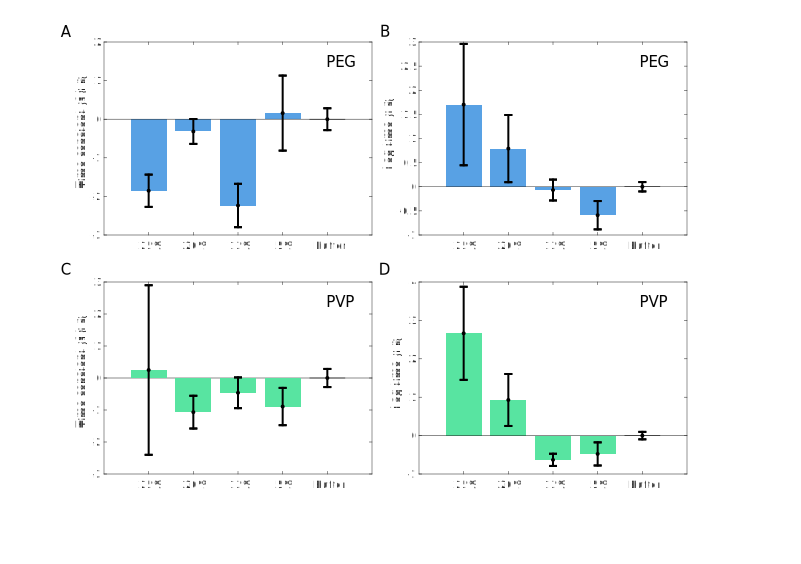
\includegraphics[width=\textwidth]{figs/ch05/peg-and-pvp-charts.pdf}
\label{fig:peg-pvp}
\end{figure}

% The ANOVA for the PEG time constants gave $p=0.0024$ with the t-test showing differences between: buffer-25\% PEG, buffer-13\% PEG, and 25\% PEG-20\% PEG. The ANOVA for the PEG lag times was likewise significant with $p = 0.0102$.  The significant pairs were: buffer-25\% PEG, buffer-20\% PEG, buffer-5\% PEG, and 25\% PEG-13\% PEG.

%For PVP, there were no significant differences in the time constant.  For the lag time, after the ANOVA and t-tests, there were differences between: buffer and everything except 5\% PVP, 25\% PVP and everything but 20\% PVP, and 20\%PVP-13\% PVP.

%For both conditions, it looks roughly like the lag time increases with the crowder concentration, but given the large error bars, I wouldn't read too much into it.  The time constants don't follow any particular trend and are mostly indistinguishable anyway.

\subsection{Discussion}

The results of the FG124 aggregation timecourses were difficult to interpret.  The reproducibility of thioflavin T fluorescence assays is notoriously poor, and many timecourses were run with high variability in results.  Results became more reproducible once the protocol was modified to include a bead in each well, which seemed to assist with mixing during the shaking incubation between time points.  Only data taken after this change are included in this dataset.

The results indicate changes in both lag time and aggregation lifetime of FG124 as a result of changing crowder conditions.  The origin and magnitude of these changes is unclear.  We chose to target the crowders PEG and PVP for further investigation.  These crowders, while typically treated as interchangeable, behaved differently in during the fluorescence timecourses (Fig.~\ref{fig:tht-all-conditions}).  When added to FG124 at a final concentration of 13\% w/v, PEG reduced the aggregation rate below that of the no-crowder condition while PVP did not.  Conversely, the lag time of the PEG condition remained approximately that of the no-crowder condition, but the lag time of the PVP condition decreased.

It is possible that the differences in aggregation time between PEG and PVP come from changes in viscosity.  The two samples do have widely different viscosity, as measured by Steve Whitten.  A 13\% PEG solution in PTB has a dynamic viscosity of 15.87 mPa s, while that of a 13\% PVP solution in PTB is 7.34 mPa s.  Studies on aggregation of insulin or $\alpha$ synuclein show varying effects of viscosity.  Increasing viscosity has been shown to increase the lag time and decrease the aggregation rate \cite{saha16,sleutel12}.  However, other studies suggest that the behavior is nonmonotonic depending on viscosity and the aggregation propensity of the protein \cite{munishkina04, magno10}.  While 13\% PEG and PVP solutions have significantly different viscosities, both fall into what Munishkina et al. define as the ``high concentration'' regime where fibrillation rate is expected to decrease \cite{munishkina04}.  The trends shown in Fig.~\ref{fig:peg-pvp} roughly agree with the supposition that crowding effects decrease lag time and increase rate for moderate crowder concentrations but have the opposite effect as viscosity effects begin to dominate.
% viscosity effects lit search LKM book 5 pg 22

To further probe the origin of the differences in aggregation, we recorded NMR spectra for FSFG and fluorescence spectra for FG124 and FSFG in crowded PEG and PVP solutions.

\section{Fluorescence spectra}

An obvious structural difference between PEG and PVP as inert crowders is the presence of an aromatic ring in PVP (Fig.~\ref{fig:peg-pvp-struct}).  The phenylalanines of FG124 also possess an aromatic ring, making ring-stacking or other interactions with PVP more likely.  As the phenylalanines are also key to transport factor binding, it is important to understand their interactions with crowders.  The presence of the ring itself makes fluorescence spectroscopy a natural choice for probing the differences between PEG and PVP as crowders.  While protein fluorescence is typically dominated by tryptophan and then tyrosine fluorescence, these amino acids are absent from both FG124 and FSFG, leaving phenylalanine with the strongest fluorescent signal.  Fluorescence spectra were therefore collected near phenylalanine's emission maximum from both fresh and aggregated FG124 in PEG or PVP.

\begin{SCfigure}
\caption[Chemical structures of PEG and PVP.]{Chemical structures of PEG and PVP (Sigma).}
\centering
\includegraphics[width=0.3\textwidth]{figs/ch05/peg-pvp-structure.pdf}
\label{fig:peg-pvp-struct}
\end{SCfigure}

\subsection{Methods}

\subsubsection{Sample preparation}
FG124 was purified as described above and in Appendix~\ref{appx:protein-purification} and stored in PTB with 7M GuHCl.  Immediately before use, 130 $\mu$L of 520 $\mu$M FG124 was desalted with a Zeba spin desalting column to remove the GuHCl.  The resulting stock was used in the crowder samples, which had a final concentration of 340 $\mu$M FG124. 

\subsubsection{Fluorescence spectra}
Fluorescence spectra were recorded using a Photon Technology International QM-6 fluorimeter.  High concentrations of crowder were not possible due to background fluorescence, so samples containing 340 $\mu$M FG124 along with 5\% w/v PEG or PVP were tested, along with FG124 in PTB only.  Blanks consisting of crowder only, buffer only, water, and FSFG in buffer were measured as well.  FG124 samples were tested before aggregation (within two hours of GuHCl removal), allowed to incubate at room temperature overnight without shaking, and tested again after aggregation.  FG124 samples were visibly cloudy after overnight incubation.

A micro quartz UV cuvette with approximately 12 $\mu$L sample volume was used for all spectra.  Between runs, the cuvette was rinsed three times with ethanol and five times with deionized water, and the exterior gently blotted with ethanol.  When aggregated FG124 was used, it was necessary to first rinse the cuvette with 7M GuHCl, soak in 7M GuHCl for five minutes, and then follow the cleaning procedure above.

The fluorimeter was set to 4 nm excitation and emission slits and an excitation wavelength of 240 nm.  Emission spectra were recorded at 1 nm intervals and automatically averaged over two runs.  The PMT detector was set to 1000 V.

\subsubsection{Data processing}
Data were normalized by averaging over two separate spectra and subtracting the appropriate blank spectrum containing the relevant crowder and buffer but no protein.

\subsection{Results}
Unfortunately, both PEG and PVP presented obstacles to the collection of UV fluorescence spectra. As shown in Fig.~\ref{fig:crowder-prop}A, PEG displayed a prominent fluorescence peak centered at 320 nm.  This may have been due to impurities in the PEG source, despite using the high-purity BioUltra brand from Sigma.  At low PEG concentrations, this peak was still small compared to that of FG124 (Fig.~\ref{fig:FG124-fresh-vs-agg}B) and could be subtracted from the signal.  However, the PEG peak limited the maximum concentration of crowder to 5\%.  PVP, on the contrary, did not display a large peak within the region of interest, but its absorbance is quite high from 240-280 nm (Fig.~\ref{fig:crowder-prop}B).  The high PEG absorbance suppresses the fluorescence signal from FG124 (Fig.~\ref{fig:FG124-fresh-vs-agg}C).  While more dramatic effects on the FG124 spectrum might be expected from higher concentrations, the limit of 5\% w/v does serve to minimize any viscosity effects.

\begin{SCfigure}
\caption[Fluorescence and absorbance of crowders.]{(A) Fluorescence spectrum of 5\% w/v PEG and 5\% w/v PVP in PTB.  Normalized by subtracting PTB spectrum.  (B) Absorbance spectrum of same samples.  Measured on a SpectraMax spectrophotometer in a cuvette with a 1 cm path length.  Normalized by subtracting PTB absorbance.}
\centering
\includegraphics[width=0.7\textwidth]{figs/ch05/crowder-properties}
\label{fig:crowder-prop}
\end{SCfigure}

Figure~\ref{fig:phe-comparison} compares the phenylalanine peaks in FSFG concat-1, fresh and aggregated FG124, and pure phenylalanine in water from \cite{prahl95}.  The phenylalanine peak slightly shifts toward longer wavelengths as the data progress from pure  phenylalanine to FSFG to fresh and aggregated FG124.  Additionally, a shoulder develops at longer wavelengths.

\begin{SCfigure}
\caption[Fluorescence spectra of FSFG, FG124, and phenylalanine.]{Fluorescence spectra of FSFG, FG124, and pure phenylalanine in water \cite{prahl95}. Excitation wavelength is 240 nm for all samples. Buffer spectra are subtracted (from FSFG and FG124 traces) and the resulting data is normalized to a maximum of one.}
\centering
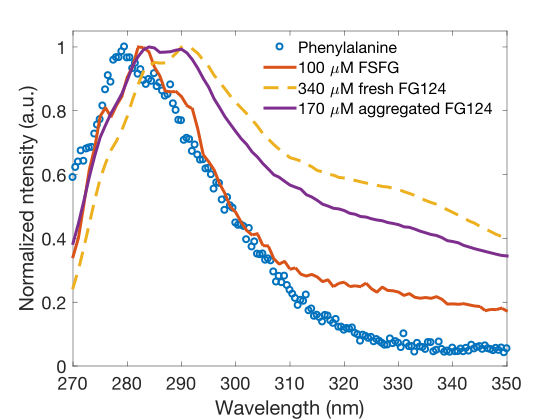
\includegraphics[width=0.4\textwidth]{figs/ch05/phe-comparison.pdf}
\label{fig:phe-comparison}
\end{SCfigure}

Fresh and aggregated FG124 samples are compared in Figs.~\ref{fig:FG124-fresh-vs-agg} and \ref{fig:stacked-FG124-fluorimetry}.  The PEG sample showed the largest difference upon aggregation, both in peak height and location.  In both crowder conditions, but not in the buffer condition, a small peak appears in the aggregated FG124 near 310 nm.

\begin{figure}
\caption[FG124 fluorescence in crowded conditions.]{Fluorescence spectra of fresh and aggregated FG124 in crowded conditions: (A) PTB buffer only, (B) 5\% w/v PEG, (C) 5\% w/v PVP.  All data normalized by subtracting appropriate blank.}
\centering
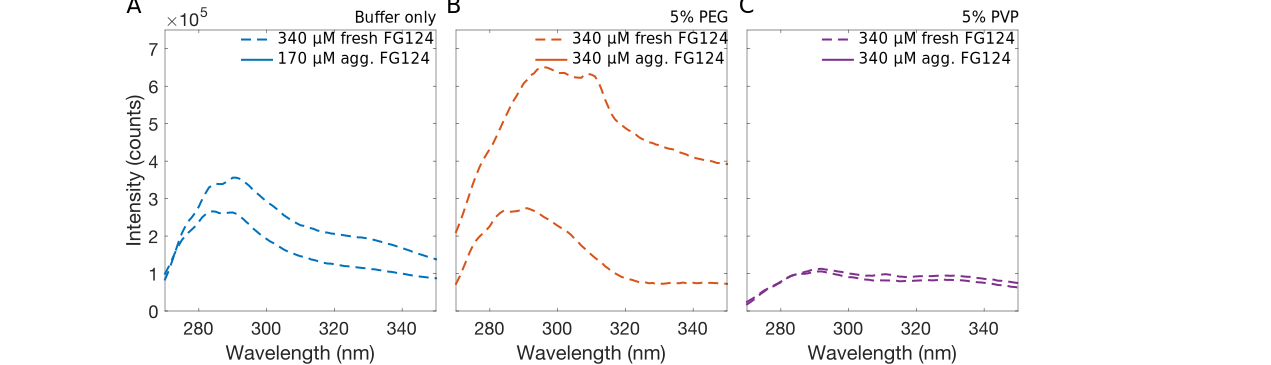
\includegraphics[width=0.9\textwidth]{figs/ch05/FG124-fresh-vs-agg.pdf}
\label{fig:FG124-fresh-vs-agg}
\end{figure}

\begin{SCfigure}
\caption[FG124 fluorescence comparison between crowding agents.]{FG124 fluorescence comparison between 5\% w/v PEG, 5\% w/v PVP, and no crowder.  All data normalized by subtracting appropriate blank and the resulting data is normalized to a maximum of one.  Traces are offset for visual clarity.\\}
\centering
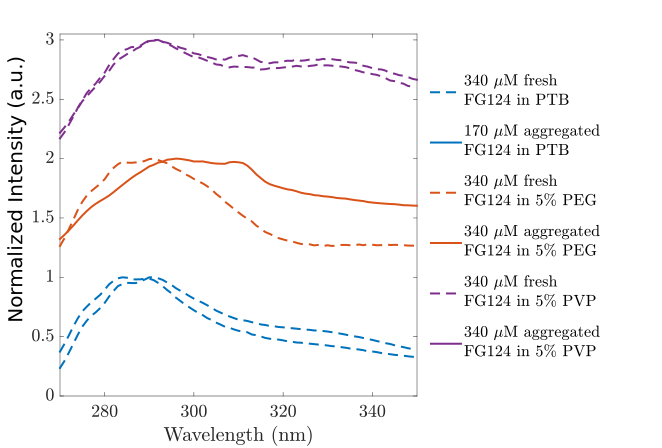
\includegraphics[width=0.6\textwidth]{figs/ch05/stacked-FG124-fluorimetry.pdf}
\label{fig:stacked-FG124-fluorimetry}
\end{SCfigure}

\subsection{Discussion}

The fluorescence spectra of proteins can in principle be used to extract many types of information, from the properties of the environment in which its aromatic residues are located to protein folding and ligand binding \cite{ladokhin00}.  This information comes from the many electronic states of the aromatic rings, which are often sensitive to the local environment and whose changes can cause shifts in fluorescence spectra.  Of the three aromatic residues, tryptophan, with its double ring, dominates a protein's fluorescence, followed by tyrosine.  Phenylalanine fluorescence is only measurable in the uncommon proteins which contain neither tryptophan or tyrosine.  Fortunately, FSFG and FG124 contain no aromatic residues except for phenylalanine.  The importance of those phenylalanine residues to binding both transport factors and other FG repeats makes them an appealing target for study by fluorimetry.  

Given the rarity of detectable phenylalanine fluorescence in proteins, little literature exists interpreting its spectral shifts.  That being the case, we can make an analogy to the tryptophan literature in broad strokes.   The complex electronic states of tryptophan give rise to a number of designated spectral classes, as shown in Fig.~\ref{fig:tryptophan}.  While very few proteins display any one of these classes in their pure form, the major trend is that the spectrum becomes redshifted when the tryptophan residue is surrounded by an increasingly hydrophilic environment \cite{ladokhin00,serrano-andres96}.  It is not clear that a similar shift should hold true in detail for phenylalanine, but it seems likely that changes in local chemical environment could lead to shifts in its emission spectrum as well.  The emergence of the smaller redshifted peaks in the spectra of the aggregated FSFG in crowded conditions, but not in the buffer sample (Fig.~\ref{fig:stacked-FG124-fluorimetry}), could well mean that the phenylalanines are interacting differently with the crowding agents.   In order to further investigate differences in the environment of the phenylalanines in crowded environments, we next measured their relaxation rates using NMR.

\begin{SCfigure}
\caption[Classes of tryptophan fluorescence.]{Qualitative depiction of spectral classes of tryptophan fluorescence. The classes correspond to differing solvent environments, with more hydrophilic environments generally being redshifted.  Figure from \cite{ladokhin00}.}
\centering
\includegraphics[width=0.4\textwidth]{figs/ch05/trytophan-ladokhin.png}
\label{fig:tryptophan}
\end{SCfigure}


\section{NMR relaxation measurements}

NMR uses the magnetic relaxation of unpaired spins, found in atoms such as 1H, 15N, and 13C to probe the local chemical environment of those spins.  When applied to isotopically labeled proteins, NMR can provide information on protein-protein interactions, structure, and relaxation rates.  Measurements of the longitudinal ($R_1$) and transverse ($R_2$) relaxation rates of each residue give information about the relaxation of individual spins and the time for the collection of spins in a sample to go out of phase with each other, respectively.  In particular, $R_2$ increases when a residue is interacting strongly with its environment.

Kathryn Wall measured the relaxation rates of FSFG in 13\% w/v PEG or PVP.  While ideally FG124 would be used, its propensity towards aggregation makes NMR experiments, which take several hours at a minimum, impossible.  Despite its differences in aggregation behavior, FSFG is a useful proxy in this case.  FSFG and FG124 are of similar lengths, derived from the Nup Nsp1, and contain similar number of FG motifs (6 FSFG motifs and 8 varied FG motifs, respectively) (Appendix~\ref{appx:sequences}).  Given that we expect the crowders to particularly affect the phenylalanines, results from FSFG are likely a good estimate of FG124 behavior as well.

\subsection{Methods}

Isotopically-labeled, his-tagged 15N FSFG was expressed in BL21DE3 Gold cells in the pRSF plasmid (Kan resistant).  Cells were grown in 1 L LB after inoculation with 1:500 preculture until reaching an OD600 of 0.6-0.8.  Cells were then pelleted by centrifuging for 10 minutes at 4000g and resuspended in a total of 1 L M9 salts pH 7.4 (10x M9 salts: 62 g/L Na$_2$HPO$_4$, 30 g/L KH$_2$PO$_4$, 5 g/L NaCl).  After washing, cells were pelleted, resuspended in 1 L M9 minimal media with 15N ammonium chloride, and induced with 1 mM IPTG for 2-4 hours.  The periplasmic matrix was then removed and the FSFG purified as described in Appendix~\ref{appx:protein-purification}.

%NMR sample prep LKM book 5 pg 10, pg 17, pg 25

The NMR samples contained 13\% w/v of either PEG or PVP, 140 $\mu$M FSFG 15N, 10\% D$_2$O, 1\% 15 mM TSP, and 1\%, 1mM DSS in PTB.  Total sample volume was 336 $\mu$L.  Ideally the protein concentration would have been at least 300 um, but the presence of the crowders reduced the available volume for protein.  An identical sample containing no crowders was also prepared.

%15N Relaxation NMR (T1/T2) % Kathryn wrote this paragraph for me
NMR experiments were run by Kathryn Wall on an Inova 600 MHz.  Using the standard 15N-HSQC experiment from the Varian BioPac, the parameter \texttt{relaxT} was adjusted for the measurement of $T_1$ and $T_2$ relaxation parameters.  For measurement of $T_1$, \texttt{relaxT} was arrayed (0, 0.1, 0.2, 0.3, 0.4, 0.5, 0.6, 0.7, 0.8, 0.9 ms).  For the measurement of $T_2$, \texttt{relaxT} was arrayed (0.01, 0.03, 0.05, 0.07, 0.09, 0.11, 0.13, 0.15, 0.17, 0.19, 0.21, 0.23, 0.25 ms).  The data was processed using standard scripts in NMRPipe, and analyzed using CCPNmr Analysis software.  


\subsection{Results}
% saved in Hough lab google drive, nuclear pore team, data, FSFG crowders

Figure~\ref{fig:NMR} shows the relaxation rates $R_1$ and $R_2$ of FSFG in 13\% PEG, 13\% PVP, or PTB without a crowder, along with the ratio $R_2/R_1$.  Due to the disordered nature of FSFG, many peaks in the NMR spectra overlap.  Amino acids of the same type experience less difference in their average local chemical environment than they would in an ordered protein, with the result that a single peak often corresponds to several amino acids.  This effect is particularly pronounced for the FSFG motif itself, in which the six repeated motifs are almost entirely collapsed to four peaks, one for each residue of the sequence.  The sole exception is the phenylalanine closest to the N-terminal, which has a peak distinct from the others.  Therefore, we broke the sequence of the FSFG peptide into quasi-repeating segments, each 19 amino acids in length, which begin with an FSFG motif and contain the hydrophilic linker which separates it from the next FSFG (Fig.~\ref{fig:NMR}B, inset).  The errors in $R_1$ and $R_2$ are given by the weighted average of the fit errors for the unique peaks that are being averaged \cite{taylor97}.  The errors of the ratio $R_2/R_1$ were propagated from $R_1$ and $R_2$ errors.

\begin{figure}
\caption[Relaxation times of FSFG in crowded conditions.]{Relaxation rates for FSFG in 13\% PEG, 13\% PVP, or PTB only.  The 19-amino-acid quasi-repeating unit that begins with the FSFG motif has been averaged over the first five repeats as shown.  Experiments performed by Kathryn Wall.  (A) Longitudinal relaxation rate $R_1$, (B) transverse relaxation rate $R_2$, (C) Ratio $R_2/R_1$.}
\centering
\includegraphics[width=\textwidth]{figs/ch05/NMR.pdf}
\label{fig:NMR}
\end{figure}

There are noticeable differences between the crowded conditions and buffer condition, which are likely due to a combination of viscosity effects and differences in interactions with the crowders.  Surprisingly, the systemic differences in rates do not all correspond to viscosity changes.  For example, the PVP sample has the highest $R_1$ and $R_2$ values overall, despite having an intermediate viscosity.  The $R_1$ values are significantly lower for the PEG sample than the other two, which also is not obviously explained by viscosity changes.

\subsection{Discussion}

There are noticeable differences between the relaxation rates in 13\% PEG, 13\% PVP, and without crowders whose source is not obvious.  In addition to varying the crowding agent, the viscosity varies from sample to sample, with buffer having the lowest and PEG the highest viscosity.  Some differences in the rates are likely due to the change in viscosity, while others may be due to differences in the peptide's interaction with the crowders.  As mentioned above, PVP shows the highest relaxation rates overall despite having an intermediate viscosity.  On the other hand, the ratio $R_2/R_1$ generally shows higher rates for PEG, then for PVP, with the lowest rates belonging to the the buffer-only sample.

\begin{SCfigure}
\caption[Approximate dependence of relaxation times on viscosity.]{Approximate dependence of relaxation times $T_1$ and $T_2$ on solvent viscosity. Figure from \cite{reich18}.}
\centering
\includegraphics[width=0.7\textwidth]{figs/ch05/viscosity-plot}
\label{fig:viscosity}
\end{SCfigure}

The typical behavior of relaxation times (with $T_1 = 1/R_1$ and $T_2 = 1/R_2$) as a function of viscosity is shown in Fig.~\ref{fig:viscosity} \cite{reich18}.  As viscosity increases, the transverse relaxation time $T_2$ decreases monotonically.  However, the longitudinal relaxation time $T_1$ begins by decreasing, reaches a turnaround point, and increases afterwards.  The location of the turnaround point $\tau_0$ is related to the strength of the NMR magnetic field expressed as a frequency $\nu_0$ by $\tau_0 = 1/\nu_0$.  For the 600 MHz instrument used in these experiments, $\tau_0 \approx 1\times 10^{-9}$ s. (Am I getting this right?)  Given that the measured rates are on the order of 1 s, $T_1$ is likely in the region where it should decrease with increasing viscosity.  In addition, the viscosities span an order of magnitude from buffer ( 1 mP s) to 13\% PEG (15 mP s), and would be expected to produce a comparably large change in relaxation rates.  Instead, the rates change by approximately 25\% at most, and the PEG sample shows the lowest relaxation rates and therefore the largest relaxation times.  Overall, the relaxation rates show features that are not obviously explained by changes in sample viscosity and may be due to differences in their interactions with the crowding agents.

\section{Conclusions}

We used several methods to investigate FG Nup aggregation in crowded conditions, focusing on FG124 as a representative peptide.  All methods indicate that there are indeed differences in aggregation and the resulting chemical environments depending on the presence and type of crowder.  The aggregation timecourses pointed to differences between most of the crowders tested, and between PEG and PVP in particular.  Since PEG and PVP are often used interchangeably as inert crowders, we pursued  these differences using fluorimetry and NMR.  Both reinforced the idea that there are in fact differences between FG124 behavior in these crowders.  The fluorescence spectra of the aggregated FG124 in particular suggests that the phenylalanines behave differently in crowded conditions than in buffer only.  Since FG repeats are involved not only to binding transport factors for selective transport, but also in forming transient crosslinks with other FG Nups, our results indicate that great care should be taken in determining what conditions to use to study Nups in vitro.
